% !TEX root = ../thesis-example.tex
%
%************************************************
% Implementierung
%************************************************
\chapter{Implementierung}
\label{sec:Implementierung}

Im letzen Kapitel haben wir unseren Reranking-Algorithmus so detailliert ausgearbeitet, dass er implementiert werden kann. In diesem Kapitel geht es nun darum diesen Algorithmus in der Springermedizin-Suche einzubauen. Mit der Implementierung wollen wir herausfinden, ob der theoretische Ansatz praktisch umgesetzt werden kann und die Gedankengänge bei der Ausarbeitung des Lösungsansatzes korrekt waren.Wir werden in diesem Kapitel nicht den Code der Lösung vorstellen. Wir werden aber beschreiben, wo wir in die Suche eingreifen, wie wir eingreifen und was wir genau machen, um dadurch einen Überblick über den implementierten Lösungsansatz schaffen zu können.

\section{Architektur der Implementierung}
\label{sec:Implementierung:Architektur}

Um zu verdeutlichen, an welcher Stelle des Suchprozesses der Springermedizin-Suche wir eingreifen, sehen wir unten folgend das Prozessbild der Implementierung unseres Lösungsansatzes. Warum wir genau an dieser Stelle eingreifen, haben wir bereits in \ref{sec:Grundlagen:Grundbegriffe:Result-RerankingPBM} ausdiskutiert. Der Suchprozess ist im Prozessbild in mehrere Komponenten aufgeteilt. Die grau hinterlegten Komponenten zeigen bereits bestehende, vom Lösungsansatz unabhängige Teile der Architektur. Die blau hinterlegten Komponenten sind die in der Implementierung neu hinzugefügte Komponenten des Lösungsansatzes. Sie sind in die drei Hauptschritte des Reranking-Algorithmus unterteilt.

\begin{figure}[H]
\centering
\vspace{-1em}
\caption[Prozessbild der Implementierung]{Prozessbild der Implementierung}
\label{fig:ProzessbildImplementierung}
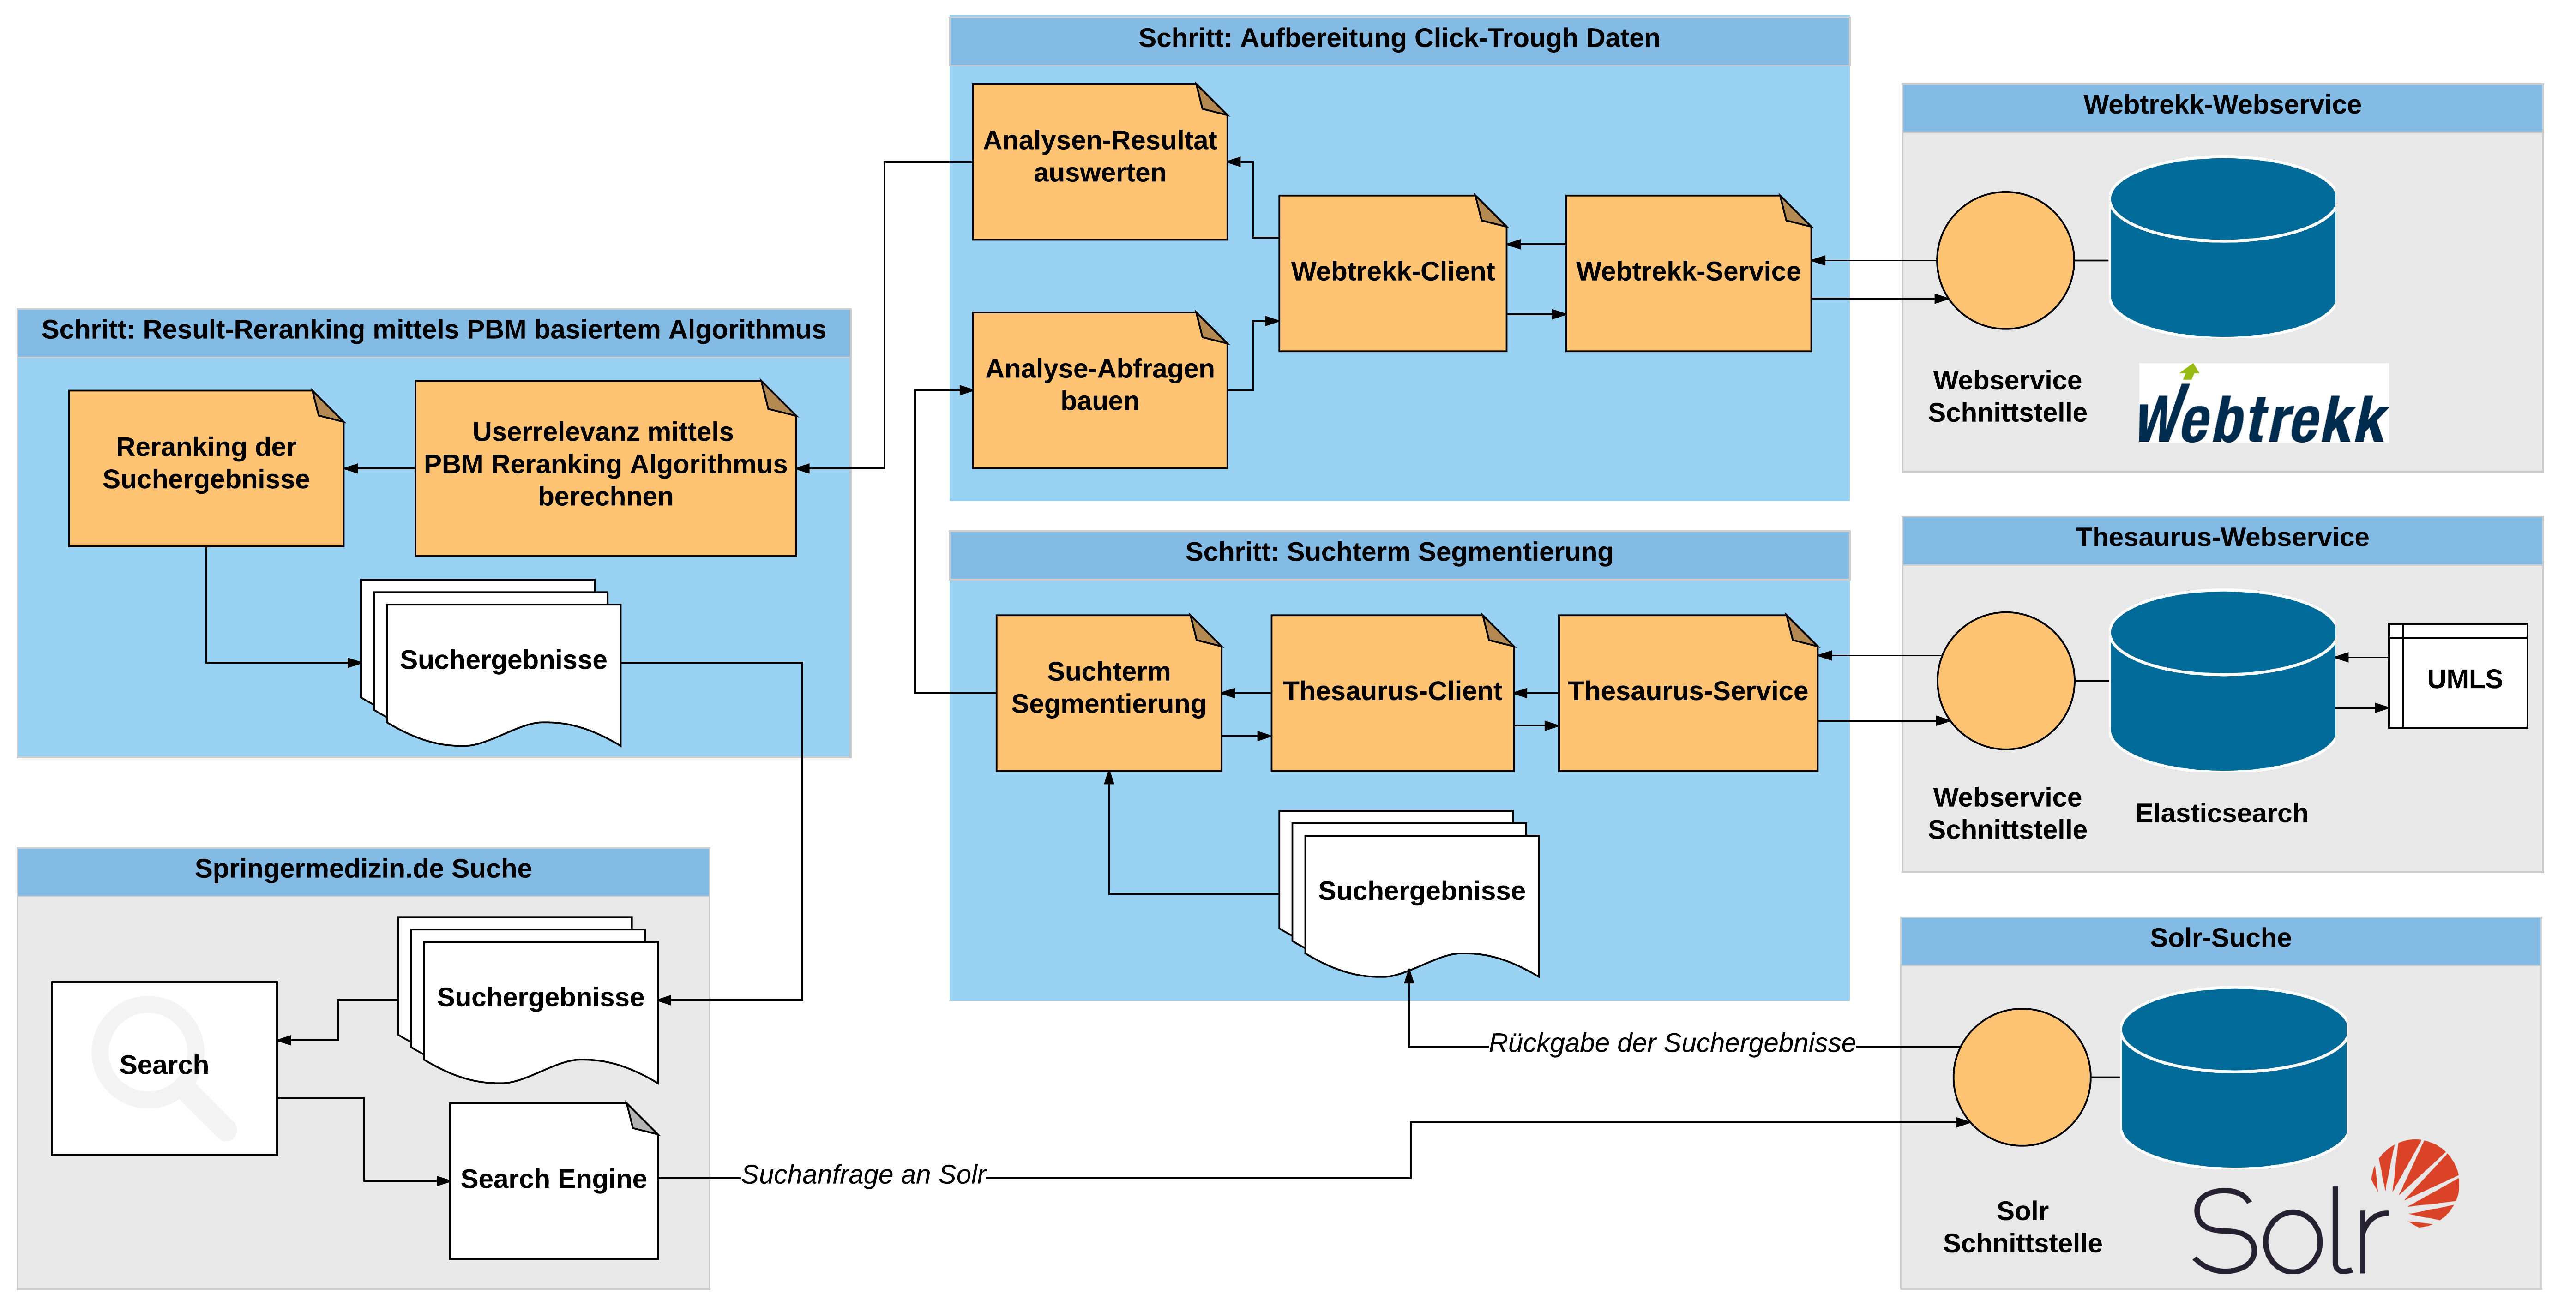
\includegraphics[width=\linewidth]{gfx/ImplementierungProzessbild}
\vspace{-3em}
\end{figure}

Wie wir in der Abbildung sehen können wird zuerst der Suchvorgang auf der Solr durchgeführt, bevor wir die Suchergebnisliste entgegennehmen, verarbeiten und mit unserem Reranking-Algorithmus neu sortieren. Die daraus resultierende Ergebnisliste geben wir dann der Suche als Suchresultat zurück. 

\paragraph{Verwendeter Technologiestack} 
Die Springermedizin-Suche ist ein Teil der White Label Applikation von Springer Nature. Diese baut auf dem MVC-Framework \textit{Play}~\cite{Play} auf und verwendet \textit{Scala}~\cite{Scala} als Programmiersprache. Unsere Implementierung wird daher in Scala geschrieben und direkt in der White Label Applikation integriert.

\section{Highlight: PBM basierter Reranking-Algorithmus}
\label{sec:Implementierung:PBM}

Der grafisch dargestellte Prozess in Abb. \ref{fig:ProzessbildImplementierung} entspricht hier nicht nicht der Reihenfolge, wie die Komponenten in der Suche aufgerufen werden, sondern der Reihenfolge der Verarbeitungsschritte im Prozess. In der effektiven Implementierung übernimmt die Reranking-Komponente die Koordination der Verarbeitungsschritte. Sie wird im Suchprozess direkt \textit{vor der Aufbereitung} der Suchergebnisse aufgerufen und nimmt die Liste der Suchergebnisse der Solr entgegen. Sind alle Schritte des Reranking-Algorithmus verarbeitet, gibt die Reranking-Komponente die \textit{neu sortierte Liste} der Suchergebnisse zurück. Diese wird dann wieder von der Springermedizin-Suche für die Ausgabe als Suchergebnisse aufbereitet.

\subsubsection{Pseudo-Code der Reranking-Komponente}
\label{sec:Implementierung:PBM:Pseudocode}

Um den angesprochenen Vorgang des Rerankings der Suchergebnisse besser zu verstehen, sehen wir hier folgend den Programm-Ablauf der Reranking-Komponente als Pseudo-Code beschrieben:

\begin{figure}[H]
\centering
\vspace{-1em}
\caption[Pseudo-Code Reranking-Algorithmus]{Pseudo-Code Reranking-Algorithmus}
\label{fig:PseudcodeRerankingAlgorithmus}
\vspace{.5em}
\DontPrintSemicolon
\begin{algorithm}[H]
\caption{PBM basierter Reranking-Algorithmus}
\BlankLine
\Daten{$searchTerm$ (Suchterm der Suchanfrage), $searchResult$ (zu verarbeitende Suchergebnisliste)}
\Ergebnis{$rerankedSearchResult \leftarrow$ durch Reranking-Algorithmus sortierte Suchergebnisliste}
\BlankLine

\Begin{
	$keywords \leftarrow$ Segmentiere und erweitere Suchterm mittels Thesaurus\;
	$ctrClickDataBySearchTerm \leftarrow$  Lese Click-Through-Daten aus Webtrekk mithilfe von $keywords$\;

	\BlankLine
	\eIf{$ctrClickDataBySearchTerm$ ist gefüllt}{
		\BlankLine
		$ranks \leftarrow$ Lese die angeklickten Positionen aus  $ctrClickDataBySearchTerm$\;
		$ctrClickDataByRanks \leftarrow$ Lese Click-Through-Daten aus Webtrekk mithilfe von $ranks$\;
		
		\BlankLine
		\eIf{$ctrClickDataByRanks$ ist gefüllt}{
			\BlankLine
			\tcc{Berechne Klick-Wahrscheinlichkeit $P(C_{u})$ aller Dokumente $u$}
			\For{ $u \in searchResult$}{
				$\lambda \leftarrow$ Definiere $\lambda$ anhand des vordefinierten Gewichtungsfaktors für die Position $r$ des Dokumentes $u$\;
				$P(E_{r_{u}}) \leftarrow$ Berechne Klick-Wahrscheinlichkeit für Position $r$ des Dokumentes $u$\;
				$P(A_{u}) \leftarrow$ Berechne Klick-Wahrscheinlichkeit für Dokument $u$ zu Suchterm $searchTerm$\;
				\BlankLine
    			$P(C_{u}) \leftarrow \lambda\cdot P(E_{r_{u}}) + (1 - \lambda)\cdot P(A_{u})$\; 
			}
			$ranksByClickProbability \leftarrow$ Sortiere Liste $searchResult$ anhand der $P(C_{u})$-Werte
			
			\BlankLine
			\tcc{Berechne Zufallswert $X_{u}$ aller Dokumente $u$}
			\For{ $u \in searchResult$}{
    			$X_{u} \leftarrow$ Berechne Zufallswert zwischen 1 und $maxPosition(searchResult)$\; 
			}
			$ranksByRandomValue \leftarrow$ Sortiere Liste $searchResult$ anhand der $X_{u}$-Werte
			
			\BlankLine
			\tcc{Berechne effektiven Relevanz-Wert $R_{u}$ aller Dokumente $u$}
			\For{ $u \in searchResult$}{
				$\lambda \leftarrow$ Definiere $\lambda$ anhand des vordefinierten Gewichtungsfaktors für den Zufallswert $X_{u}$\;
				$r_{P(C_{u})} \leftarrow$ Lese Position des Wahrscheinlichkeits-Wertes $P(C_{u})$ aus $ranksByClickProbability$\;
				$r_{X_{u}} \leftarrow$ Lese Position des Zufallswertes $X_{u}$ aus $ranksByRandomValue$\;
				\BlankLine
    			$R_{u} \leftarrow 1 / \left(\lambda\cdot r_{X_{u}} + (1 - \lambda)\cdot r_{P(C_{u})}\right)$\;
			}
			$rerankedSearchResult \leftarrow$ Sortiere Liste $searchResult$ anhand der $R_{u}$-Werte\;
			\tcc{Rückgabe der durch den Reranking-Algorithmus umsortierten Suchergebnisse}
			\KwRet{die ersten 20 Elemente von $rerankedSearchResult$}
		}{	
			\tcc{Keine Click-Through-Daten für die angeklickten Positionen gefunden $\Rightarrow$\\
			Keine Umsortierung der Suchergebnisse mit dem Reranking-Algorithmus}
			\KwRet{die ersten 20 Elemente von $searchResult$}
		}
	}{
		\tcc{Keine Click-Through-Daten für Suchterm gefunden $\Rightarrow$\\
		Keine Umsortierung der Suchergebnisse mit dem Reranking-Algorithmus}
		\KwRet{die ersten 20 Elemente von $searchResult$}
	}
}
\end{algorithm}
\end{figure}

\section{Highlight: Webtrekk-Analysen}
\label{sec:Implementierung:Webtrekk}

Wie in der Einführung dieser Arbeit in \ref{sec:Einfuehrung:AufbauSucheBeiSpringerNature:Webtrekk} angesprochen, speichert Springermedizin seine Tracking-Daten auf Webtrekk. Für die Implementierung des Reranking-Algorithmus müssen wir die Click-Through-Daten für die Wahrscheinlichkeits-Berechnungen, wie in \ref{sec:Reranking:Methodik:Result-RerankingPBM} besprochen, mithilfe von Analysen aus Webtrekk abfragen und auswerten. Wie wir diese Analysen abfragen, sehen wir folgend.

\subsubsection{Abfrage von Analysen}
\label{sec:Implementierung:Webtrekk:AnalysenAbfragen}

Der Webservice von Webtrekk bietet verschiedene Schnittstellenmethoden zum Export und Herunterladen der Tracking-Daten an. Die für uns relevante Schnittstellenmethode lautet \textit{getAnalysisData}. Mithilfe dieser Methode können die Daten der verschiedenen Analysen per REST-Schnittstelle\footnote{Representational State Transfer, ist ein Architekturmodell mit dem Webservices mit den Standard-HTTP-Methoden (GET, POST, PUT und DELETE) realisiert werden können} abgerufen werden. Um zu definieren, welche Analyse und mit welchen Filtern diese Analyse abgefragt werden soll, müssen wir folgende Parameter der Methode mitgeben: 

\textbf{Request:} \textit{Springermedizin-Suche $\rightarrow$ Webtrekk REST-Webservice}

\begin{table}[H]
\centering
\vspace{-.75em}
\caption[Beschreibung Analyse-Aufbau Webtrekk-Schnittstelle]{Beschreibung Analyse-Aufbau Webtrekk-Schnittstelle}
\vspace{-.5em}
\label{tab:BeispielCTDaten}
\footnotesize
\renewcommand*{\arraystretch}{1.2}
\resizebox{\textwidth}{!}{%
\begin{tabular}{ll}
\hline
\textbf{Parameter}   & \textbf{Beschreibung}                                                                              \\ \hline
\textit{analysis}    & Gewünschte Analyse (alle Analysen der Weboberfläche von Webtrekk sind so abrufbar)                  \\
\textit{time\_start} & Startzeit des Analysezeitraumes                                                                    \\
\textit{time\_stop}  & Stopzeit des Analysezeitraumes                                                                     \\
\textit{column}               & Ausgabe bestimmter, in der Standard-Analyse nicht vorhandener Datenspalten                           \\
\textit{analysis\_filter}     & Komplexe Filter bestehen aus einem oder mehreren Filtern, die logisch miteinander verknüpft werden \\ \hline
\end{tabular}
}
\vspace{-2em}
\end{table}

Zur Berechnung der Klick-Wahrscheinlichkeiten benötigen wir zwei verschieden Analysen. Beispiel-Anfragen für diese beiden Analysen sehen wie folgt aus:

\textbf{Suchanfrage:} \textit{Krebs $\rightarrow$ Springermedizin-Suche}

\begin{table}[H]
\centering
\vspace{-.75em}
\caption[Beispiel Analyse-Aufbau Webtrekk-Schnittstelle]{Beispiel Analyse-Aufbau Webtrekk-Schnittstelle}
\vspace{-.5em}
\label{tab:BeispielCTDaten}
\footnotesize
\renewcommand*{\arraystretch}{1.2}
\resizebox{\textwidth}{!}{%
\begin{tabular}{lll}
\hline
\textbf{Parameter}        & \textbf{Wahrscheinlichkeit $P(A_{u})$}                                                                                                                                                            & \textbf{Wahrscheinlichkeit $P(E_{r_{u}})$}                                                                                                                              \\ \hline
\textit{analysis}         & Navigation|Events                                                                                                                                                                                & Navigation|Events                                                                                                                                                      \\ \hline
\textit{time\_start}      & 2016-08-01                                                                                                                                                                                       & 2016-08-01                                                                                                                                                             \\ \hline
\textit{time\_stop}       & 2016-08-31                                                                                                                                                                                       & 2016-08-31                                                                                                                                                             \\ \hline
\textit{column}           & {[}Page Impressions,\% Visits,Ø - Suchtreffer{]}                                                                                                                                                 & {[}Page Impressions,\% Visits,Ø - Suchtreffer{]}                                                                                                                       \\ \hline
\textit{analysis\_filter} & \begin{tabular}[c]{@{}l@{}}{[} {[},Events,LIKE,searchresult-*{]},\\ {[}AND,Internal Search Phrases,LIKE,*Krebs*{]},\\ {[}OR,Internal Search Phrases,LIKE,*Maligne Tumoren*{]} {]}\end{tabular} & \begin{tabular}[c]{@{}l@{}}{[} {[},Events,LIKE,searchresult-1.*{]},\\ {[}OR,Events,LIKE,searchresult-4.*{]},\\ {[}OR,Events,LIKE,searchresult-29.*{]} {]}\end{tabular} \\ \hline
\end{tabular}
}
\vspace{-2em}
\end{table}

In der Antwort für diese Analysen werden die Click-Through-Daten als JSON-Array\footnote{Die JavaScript Object Notation (JSON) ist ein kompaktes Format zum Austausch von Daten} zurückgegeben. Wie der ausgewertete JSON-Array aussehen kann, haben wir in Kapitel \ref{sec:Grundlagen:Grundbegriffe:Click-Through-Daten:AussehenClick-Through-Daten} angeschaut. 


\section{Zusammenfassung}
\label{sec:Implementierung:Zusammenfassung}

In diesem Kapitel haben wir eine Übersicht über die Architektur und die wichtigsten Highlights der Implementierung gekriegt. Wir wissen nun \textit{wie} der Lösungsansatz des Reranking-Algorithmus implementiert werden kann. Verknüpfen wir dieses Wissen mit dem aus Kapitel \ref{sec:Reranking}, könnten wir den Reranking-Algorithmus nun auch auf eine andere Suche adaptieren. Im nächsten Kapitel wollen wir nun, mithilfe der implementierten Suche evaluieren, welche Verbesserung für das Qualitätsmaß der Suche von Springermedizin der Lösungsansatz bringt.